\documentclass[12pt,oneside,a4paper]{ctexart}
\usepackage{geometry}
\geometry{left=3.0cm, right=3.0cm, top=4.0cm, top=4.0cm}
\usepackage{booktabs}
\usepackage{float}
\usepackage{fontspec}
\usepackage{amsmath}
\usepackage{graphicx}
\usepackage{tikz}
\usepackage{mathpazo}
\usepackage{listings}
\usepackage{xcolor}
\usepackage{indentfirst}
\begin{document}

\lstset{numbers=left,
	tabsize=4,
	frame=single,
	xleftmargin=1em,
	basicstyle=\fontspec{Consolas},
	numberstyle=\fontspec{Consolas},
	showstringspaces=false,
	breaklines,
	keywordstyle= \color{ blue!70},
	commentstyle=\color{red!50!green!50!blue!50},
	rulesepcolor= \color{ red!20!green!20!blue!20}
}

\title{计算机图形学 \\ 课程项目}
\author{ 王徐笑风\thanks{学号:18120193 E-mail:2208740924@qq.com}
	\and 凌泽辉\thanks{学号:18120193 E-mail:785896610@qq.com}}
\date{\today}
\maketitle
\newpage
\tableofcontents
\newpage
\begin{abstract}
	查找资料,学习了解三维网格模型的相关知识。完成一个三维网格模型的显示系统。

	数据输入:通过文件读取模型数据

	数据存储:设计程序内用于存储模型数据的数据结构

	数据输出:在窗口界面进行模型显示

	编程实现三维到二维的投影变换计算

	编程实现通过键盘或鼠标驱动模型的平移、缩放及旋转变换

	可以使用开发工具中提供光照函数,若自己编程实现光照计算,则可获得额外加分
\end{abstract}

\section{三维图形的变换与表示}
\subsection{向量与点}
在三维空间中我们常用一个三维向量表示一个点,虽然向量本身只表达长度和方向,他是无关坐标系的,
而点显然是与选取的坐标系是相关的。因此在这里将点理解为在一个给定的坐标系下,原点按某一向量移动后的位置,它写作式(\ref{Point}):
\begin{equation}
	\mathbf{P} = \begin{bmatrix}
		x \\
		y \\
		z
	\end{bmatrix}
	\label{Point}
\end{equation}
\subsection{变换}
对于三维空间中的点,常用到的仿射变换和二维中的类似:平移、旋转和缩放。
\subsubsection{平移}
平移变换是将一个点按一个方向,移动一段距离。考虑到上面我们的点的定义即为在给点的坐标系下,原点按一个向量移动的距离。那么显然平移一个点即将原点平移两次,即点所代表的“向量”和平移向量的共同作用。

对于点$\mathbf{P}$,将其平移$\mathbf{V}$:
\begin{equation*}
	\mathbf{P}=
	\begin{bmatrix}
		\mathbf{P}_x \\
		\mathbf{P}_y \\
		\mathbf{P}_z
	\end{bmatrix}
\end{equation*}
\begin{equation*}
	\mathbf{V}=
	\begin{bmatrix}
		\mathbf{V}_x \\
		\mathbf{V}_y \\
		\mathbf{V}_z
	\end{bmatrix}
\end{equation*}

则有平移后的点$\mathbf{N}$:
\begin{equation*}
	\mathbf{N}=
	\begin{bmatrix}
		\mathbf{P}_x \\
		\mathbf{P}_y \\
		\mathbf{P}_z
	\end{bmatrix}+\begin{bmatrix}
		\mathbf{V}_x \\
		\mathbf{V}_y \\
		\mathbf{V}_z
	\end{bmatrix} =
	\begin{bmatrix}
		\mathbf{P}_x + \mathbf{V}_x \\
		\mathbf{P}_y + \mathbf{V}_y \\
		\mathbf{P}_z + \mathbf{V}_z
	\end{bmatrix}
\end{equation*}
\subsubsection{旋转}
旋转指的是:点以三维空间中的某点为旋转中心,进行旋转,这里简略的认为旋转中心为坐标系原点,即此时的旋转变换是一个特殊的线性变换。
在三维坐标系中对点做按原点的旋转,即是对一个向量进行旋转。只需要求取原基向量 $\hat{i}$、$\hat{j}$、$\hat{k}$ ,在旋转后的 $\hat{i'}$、$\hat{j'}$、$\hat{k'}$,可以得到旋转矩阵:
\begin{equation*}
	\mathbf{RotateMatrix} =
	\begin{bmatrix}
		\hat{i'_x} & \hat{j'_x} & \hat{k'_x} \\
		\hat{i'_y} & \hat{j'_y} & \hat{k'_y} \\
		\hat{i'_z} & \hat{j'_z} & \hat{k'_z}
	\end{bmatrix}
\end{equation*}

则有旋转后的点$\mathbf{N}$:
\begin{equation*}
	\mathbf{N} = \begin{bmatrix}
		\hat{i'_x} & \hat{j'_x} & \hat{k'_x} \\
		\hat{i'_y} & \hat{j'_y} & \hat{k'_y} \\
		\hat{i'_z} & \hat{j'_z} & \hat{k'_z}
	\end{bmatrix} \times \begin{bmatrix}
		\mathbf{P}_x \\
		\mathbf{P}_y \\
		\mathbf{P}_z
	\end{bmatrix}
\end{equation*}

特别的,绕Y轴旋转 $\theta$ 弧度的旋转矩阵,可以这么考虑:首先Y轴显然是不变的,在左手系下从Y轴逆方向向下看,Z轴X轴正好组成一个平面直角坐标系。则 $\hat{i}$ 顺时针旋转过 $\theta$ 弧度后的向量为:
\begin{equation*}
	\hat{i'}=\begin{bmatrix}
		cos(\theta)  \\
		0            \\
		-sin(\theta) \\
	\end{bmatrix}
\end{equation*}

同样的 $\hat{k}$ 旋转过 $\theta$ 弧度后的向量为:
\begin{equation*}
	\hat{k'}=\begin{bmatrix}
		sin(\theta) \\
		0           \\
		cos(\theta) \\
	\end{bmatrix}
\end{equation*}

综上,Y轴旋转矩阵为:
\begin{equation}
	\mathbf{RotateY}(\theta)=\begin{bmatrix}
		cos(\theta)  & 0 & sin(\theta) \\
		0            & 1 & 0           \\
		-sin(\theta) & 0 & cos(\theta)
	\end{bmatrix}
	\label{RotateY}
\end{equation}

类似的我们也可以得到X轴旋转和Z轴旋转矩阵:
\begin{equation}
	\mathbf{RotateX}(\theta)=\begin{bmatrix}
		1 & 0           & 0            \\
		0 & cos(\theta) & -sin(\theta) \\
		0 & sin(\theta) & cos(\theta)
	\end{bmatrix}
	\label{RotateX}
\end{equation}

\begin{equation}
	\mathbf{RotateZ}(\theta)=\begin{bmatrix}
		cos(\theta) & -sin(\theta) & 0 \\
		sin(\theta) & cos(\theta)  & 0 \\
		0           & 0            & 1
	\end{bmatrix}
	\label{RotateZ}
\end{equation}

最后,通过上述(\ref{RotateX})、(\ref{RotateY})、(\ref{RotateZ})的旋转矩阵的复合矩阵即可实现任意的旋转,即:
\begin{equation*}
	\mathbf{Rotate}(\alpha,\beta,\gamma)=\mathbf{RotateZ}(\gamma)\times{}\mathbf{RotateY}(\beta)\times{}\mathbf{RotateX}(\gamma)
\end{equation*}
\subsubsection{缩放}

缩放的实现和旋转矩阵类似,计算出新的 $\hat{i'}$、$\hat{j'}$、$\hat{k'}$ 即可:
\begin{equation*}
	\mathbf{Scale}(\alpha,\beta,\gamma)=\begin{bmatrix}
		\alpha & 0     & 0      \\
		0      & \beta & 0      \\
		0      & 0     & \gamma
	\end{bmatrix}
\end{equation*}

则缩放后的点为:
\begin{equation*}
	\mathbf{N}=\begin{bmatrix}
		\alpha & 0     & 0      \\
		0      & \beta & 0      \\
		0      & 0     & \gamma
	\end{bmatrix}
	\times
	\begin{bmatrix}
		x \\
		y \\
		z
	\end{bmatrix}=
	\begin{bmatrix}
		\alpha{}x \\
		\beta{}y  \\
		\gamma{}z
	\end{bmatrix}
\end{equation*}

\subsubsection{复合变换}
不难看出上述的变换中,旋转和缩放的变换可以简单地实现符合,将旋转矩阵和缩放矩阵进行矩阵乘法复合即可,同时这里两者是可交换的。

但平移变换就无法使用矩阵表达(矩阵变换后的点 $\mathbf{N}$ 的一个分量可以表达为 $\mathbf{N}_x=a\mathbf{P}_x+b\mathbf{P}_y+c\mathbf{P}_z$ 而平移变换可表达为 $\mathbf{N}_x=\mathbf{P}_x+d$ 显然上述公式中 $a=1, \mathbf{P}_y+c\mathbf{P}_z=d$ 显然无法使用一个静态的矩阵实现),因此在描述一个点的平移、旋转和缩放变换时,我们使用下述公式(\ref{Transform_All})
\begin{equation}
	\mathbf{N}=
	(
	\mathbf{Scale}(a,b,c)
	\times
	\mathbf{Rotate}(\alpha,\beta,\gamma)
	)\times
	\mathbf{P}
	+
	\mathbf{V}
	\label{Transform_All}
\end{equation}

但使用上述公式计算是不“简单”的,我们希望能有一种方法通过一次一种计算即可表达上述三种变换,同时又能提高运算的效率。
\subsection{三维的齐次坐标}
在三维中我们无法将平移、旋转和缩放变换由一个矩阵描述。不妨假设我们在四维中,并规定点 $\mathbf{P}$ 在四维中的坐标为:
\begin{equation*}
	\mathbf{P}=
	\begin{bmatrix}
		x \\
		y \\
		z \\
		w=1
	\end{bmatrix}
\end{equation*}

即对于 $\forall{}\mathbf{P}$ 他们位于四维空间中分量 $w=1$ 的一个三维“切片”空间中。

有了三维其次坐标后,我们可以改写公式(\ref{Transform_All})为:
\begin{equation}
	\mathbf{N} =
	\begin{bmatrix}
		a & b & c & d \\
		e & f & g & h \\
		i & j & k & l \\
		0 & 0 & 0 & 1
	\end{bmatrix}_{\mathbf{Transform}}
	\times
	\begin{bmatrix}
		x \\
		y \\
		z \\
		1
	\end{bmatrix}_{\mathbf{P}}
	=
	\begin{bmatrix}
		ax+by+cz+d \\
		ex+fy+gz+h \\
		ix+jy+kz+l \\
		1          \\
	\end{bmatrix}
	\label{Transform_All_New}
\end{equation}

观察公式(\ref{Transform_All_New}),其中 $d, h, l$ 显然对应了平移向量:
\begin{equation*}
	\mathbf{V}=
	\begin{bmatrix}
		d \\
		h \\
		l \\
		1
	\end{bmatrix}
\end{equation*}

它可以写成一个平移矩阵:
\begin{equation}
	\mathbf{Translate}=
	\begin{bmatrix}
		1 & 0 & 0 & d \\
		0 & 1 & 0 & h \\
		0 & 0 & 1 & l \\
		0 & 0 & 0 & 1 \\
	\end{bmatrix}
	\label{Translate_Matrix}
\end{equation}

而将平移矩阵和旋转缩放矩阵复合即可得到公式(\ref{Transform_All_New})中的变换矩阵:
\begin{align}
	\mathbf{Translate}\times \mathbf{Scale}\times \mathbf{Rotation}= &
	\begin{bmatrix}
		1 & 0 & 0 & d \\
		0 & 1 & 0 & h \\
		0 & 0 & 1 & l \\
		0 & 0 & 0 & 1 \\
	\end{bmatrix}_{\mathbf{Translate}}
	\times
	\begin{bmatrix}
		a & b & c & 0 \\
		e & f & g & 0 \\
		i & j & k & 0 \\
		0 & 0 & 0 & 1
	\end{bmatrix}_{\mathbf{Scale}\times \mathbf{Rotation}}         \notag                                       \\
	=                                                                & \begin{bmatrix}
		a & b & c & d \\
		e & f & g & h \\
		i & j & k & l \\
		0 & 0 & 0 & 1
	\end{bmatrix}_{\mathbf{Transform}}\notag
\end{align}

综上我们通过三维空间中的齐次坐标实现了3种变换的复合。当然 $Transform$ 矩阵也能表达切变等仿射变换,由于在三维投影的过程中并不常用,这里就不详细叙述。

\subsubsection{$sunMatLib.h$ 矩阵运算库}
在本项目中,除了窗口创建和像素绘制使用到了第三方软件库,所有的数据结构、矩阵矩阵运算、投影、光栅化、光照等都有我们小组自己实现。这里简单介绍一下整个项目中频繁使用到的矩阵运算类库,见源码:
\newline
\begin{lstlisting}[language=c++]
class Vector3
{
	friend class Matrix4;
	
public:
	double _x, _y, _z, _w;
	
public:
	Vector3();
	Vector3(const double &x, const double &y, const double &z);
	Vector3(const Vector3 &copy);
	
	Vector3 &operator=(const Vector3 &copy);
	Vector3 operator+(const Vector3 &b) const;
	Vector3 operator-(const Vector3 &b) const;
	Vector3 operator*(const double &a) const;
	friend Vector3 operator*(const double &a, const Vector3 &b);
	double operator*(const Vector3 &b) const;
	Vector3 &operator*=(const double &a);
	Vector3 &operator+=(const Vector3 &b);
	friend Vector3 operator/(const Vector3 &b, const double &a);
	friend Vector3 &operator/=(Vector3 &b, const double &a);
	double length() const;
	Vector3 normalize() const;
	Vector3 &normalized();
	Vector3 cross(const Vector3 &b) const;
	Vector3 &crossed(const Vector3 &b);
	Vector3 &set(const double &x, const double &y, const double &z);
	
	static Vector3 ONE();
	static Vector3 ZERO();
	static Vector3 UP();
	static Vector3 FRONT();
	static Vector3 RIGHT();
};
\end{lstlisting}
\begin{lstlisting}[language=c++]
class Matrix4
{
	friend class Vector3;

	private:
	double _mat[4][4];

	public:
	Matrix4();
	Matrix4(double copy[4][4]);
	Matrix4(const Matrix4 &copy);

	Matrix4 quickInvert();
	Matrix4 &operator=(const Matrix4 &copy);
	Matrix4 operator*(const Matrix4 &b);
	Vector3 operator*(const Vector3 &b);

	static Matrix4 PROJECTION(const double &aspect_ratio, const double &fov_rad, const double &near_panel, const double &far_panel);
	static Matrix4 ROTATE_X(const double &angle);
	static Matrix4 ROTATE_Y(const double &angle);
	static Matrix4 ROTATE_Z(const double &angle);
	static Matrix4 ROTATE(const double &x, const double &y, const double &z);
	static Matrix4 SCALE(const double &x, const double &y, const double &z);
	static Matrix4 TRANSLATE(const double &x, const double &y, const double &z);
	static Matrix4 POINTAT(Vector3 pos, Vector3 target, Vector3 up);
};
\end{lstlisting}

\subsection{三角面}
虽然三维形体有很多表示方法,但在三维的渲染引擎或是游戏引擎中,最常使用到的还是三角网格模型。

在这种网格模型中一个面一个三维空间中的三角面,它由3个顶点 $\mathbf{P}_1,\mathbf{P}_2, \mathbf{P}_3$ 即可表达。

保留法向信息,三角化的 $.obj$ 文件就是这样一种三角网格模型,在本项目中也该文件格式作为标准。

特别的,在三维渲染中,单个三角面往往还有“朝向”这一属性。背对我们的三角面是不显示的,只有面对我们的才会渲染。这种规定在处理封闭模型和时候会更加有效:首先我们是无法看到封闭模型的内部的,自然无需渲染其三角面的背面;第二,背对我们的三角面不进行渲染也能降低对于性能的需求。因此三角面还存在一个法向量,它垂直于三角面所在的平面,并与三角面朝向同向。

但这不代表我们需要使用除3个三维点以外的数据保存法向信息。在 $.obj$ 中一个三角面 $face$ 由3个顶点 $vertex$ 组成。这三个顶点按原三角面的逆时针排列,其法向满足右手螺旋定则,因此对于1个三角面的有序顶点 $\mathbf{P}_1,\mathbf{P}_2, \mathbf{P}_3$ ,该三角面的单位法向量 $\mathbf{U}$ 为:
\begin{equation*}
	\mathbf{U}=
	\frac{(\mathbf{P}_2 - \mathbf{P}_1)\times
		(\mathbf{P}_3 - \mathbf{P}_1)}{\left\lvert (\mathbf{P}_2 - \mathbf{P}_1)\times
		(\mathbf{P}_3 - \mathbf{P}_1)\right\rvert }
\end{equation*}

在 $sunMatLib.h$ 也有三角面类 $TriFace$ ,它实现了法向的自动计算,在通过顶点构造了三角面后,即可通过 $get_Normal()$ 方法获得单位法向量。具体实现可见源程序代码。
\subsection{网格}
在有了三角面的数据结构后,三角网格模型的最简单的实现就是使用变长数组保存每一个三角面。

在 $sun3D.h$ 中的 $Mesh$ 类就是使用了 $std::vector<TriFace>$ 来保存三角网格模型。
\subsubsection{$.obj$ 文件的加载}

$.obj$ 文件的构成或是说格式,基本上一一对应了上述的三角面、三角网格模型的数据结构。我们先来看一个  $.obj$ 文件实例($untitled1.obj$ 文件有省略):
\newline
\begin{lstlisting}
# Blender v2.83.4 OBJ File: ''
# www.blender.org
o Torus
v 1.250000 0.000000 0.000000
v 1.216506 0.125000 0.000000
v 1.125000 0.216506 0.000000
v 1.000000 0.250000 0.000000
......
s off
f 13 2 1
f 2 15 3
f 15 4 3
f 16 5 4
......
\end{lstlisting}

其中“\#”开头的是注释,忽略即可。

“v” 开头的一行定义了一个顶点,后跟三个数值分别表示该顶点 $\mathbf{P}$ 的 $x, y, z$ 分量

“f” 开头的一行定义了一个三角面,后跟三个整数分别表示该三角面的3个顶点 $\mathbf{P}_1, \mathbf{P}_2, \mathbf{P}_3$ 所对应的顶点“v”的序号。例如:上述文件中的第10行 “f 13 2 1”,其中 “2 1” 表明 $\mathbf{P}_2$ 为第5行的顶点, $\mathbf{P}_3$ 为第4行的顶点。

因此,读取 $.obj$ 文件十分简单,设置一个 $std::vector<Vector3>$ 来保存顶点,当读取到一行以“v”开头就构造一个 $Vector3$ 顶点,并放入 $std::vector<Vector3>$ 中,当读取到一行以“f”开头就从 $std::vector<Vector3>$ 中依次取出相应下标的顶点,构造三角面,并放入需要的 $Mesh$ 实例中的 $std::vector<TriFace>$ 即可。
\section{投影}
想要实现三维模型的显示,最重要的是找到一种将三维模型“转换”/“映射”/“投影”到二维平面的方法。

当然我们需要规定一下这个投影后的二维平面的格式。一般的,在我们的程序中,屏幕的标准坐标系为:从左到右为X轴方向 $[-1,1]$ ,从下到上为Y轴方向 $[-1,1]$ 。

自然的,根据上述定义,采用左手系,可以得到Z轴方向为从屏幕外指向屏幕内部,这也是我们的摄像机的朝向。
\subsection{正交投影}

一种简单的投影方式是“正交投影”。它几乎可以简单的理解为:忽略三维点的 $z$ 分量,直接将 $x, y$ 分量和屏幕坐标相关联。因此,正交投影是“忽略透视的”,他没有消失点这一概念,在三维空间中的平行线在投影到屏幕坐标后也是保持平行的。这当然我我们的现实经验是不同的,见图(\ref{OrthVSPers})。虽然在某些场景下,正交投影的这种性质能更好地表达某些信息,但更为常用的还是“透视投影”。只因正交投影在之后介绍透视投影会有所帮助,因此在这里做简要的介绍。
\begin{figure}[H]
	\centering
	\includegraphics[scale=0.4]{Picture/Annotation 2020-06-23 205119.png}
	\vspace{-2ex}
	\caption{正交投影 $vs$ 透视投影}
	\label{OrthVSPers}
\end{figure}

在正交投影中,我们需要把某个区域内的点映射到 $[-1,1]$ 的屏幕空间中,这个区域是一个长方体,称为“视域”。它由上下左右和远近6个平面组成。
\begin{figure}[H]
	\centering
	\includegraphics[scale=0.4]{Picture/Annotation 2020-06-23 205119.png}
	\vspace{-2ex}
	\caption{正交投影 $vs$ 透视投影}
	\label{OrthViewCube}
\end{figure}

对于每个面有如下参数:
\begin{enumerate}
	\item $l =$左平面 $x$ 分量
	\item $r =$ 右平面 $x$ 分量
	\item $t =$ 上平面 $y$ 分量
	\item $b =$ 下平面 $y$ 分量
	\item $f =$ 远平面 $z$ 分量
	\item $n =$ 近平面 $z$ 分量
\end{enumerate}

在这个视域中的三维点 $\mathbf{P}$ ,其 $x$ 分量需要按照左右平面的位置映射近 $[-1,1]$ 区间,在数轴上可以如下表示:
\begin{figure}[H]
	\centering
	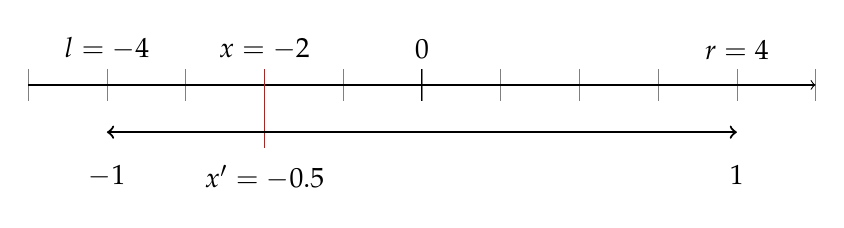
\begin{tikzpicture}[node distance=2cm]
		\draw[step=1cm,gray,very thin] (-5, -0.2) grid (5,0.2);
		\draw (-4cm, 0.2cm) node[anchor=south] {$l=-4$};
		\draw (4cm, 0.2cm) node[anchor=south] {$r=4$};
		\draw (-2cm, 0.2cm) node[anchor=south] {$x=-2$};
		\draw (0cm, 0.2cm) node[anchor=south] {$0$};
		\draw[->](-5,0)--(5,0);
		\draw[-](0,-0.2)--(0,0.2);
		\draw[-,red](-2,-0.8)--(-2,0.2);
		\draw[<->,thick](-4,-0.6)--(4,-0.6);
		\draw (-4cm, -0.9cm) node[anchor=north] {$-1$};
		\draw (4cm, -0.9cm) node[anchor=north] {$1$};
		\draw (-2cm, -0.9cm) node[anchor=north] {$x'=-0.5$};
	\end{tikzpicture}
	\caption{$x$ 分量,与 $l,r$ 的映射关系}
	\vspace{-2ex}
\end{figure}

显然的, $x$ 分量的映射公式为:
\begin{equation*}
	x'=\frac{2x}{r-l}-\frac{r+l}{r-l}
\end{equation*}

同理, $y$ 分量的映射公式为:
\begin{equation*}
	y'=\frac{2y}{t-b}-\frac{t+b}{t-b}
\end{equation*}

最后, $z$ 分量的映射公式回稍有不同,因为这次我们将他映射到 $[0,1]$ 之间,而非 $[-1,1]$ 。
\begin{equation*}
	z'=\frac{z}{f-n}-\frac{n}{f-n}
\end{equation*}

不妨将上述三个公式整合入一个变换矩阵,即为正交投影矩阵:
\begin{equation}
	\mathbf{Orthogonal}=
	\begin{bmatrix}
		\frac{2}{r-l} & 0             & 0             & -\frac{r+l}{r-l} \\
		0             & \frac{2}{t-b} & 0             & -\frac{t+b}{t-b} \\
		0             & 0             & \frac{1}{f-n} & -\frac{n}{f-n}   \\
		0             & 0             & 0             & 1
	\end{bmatrix}
\end{equation}
\begin{equation*}
	\mathbf{P'}=
	\begin{bmatrix}
		\frac{2}{r-l} & 0             & 0             & -\frac{r+l}{r-l} \\
		0             & \frac{2}{t-b} & 0             & -\frac{t+b}{t-b} \\
		0             & 0             & \frac{1}{f-n} & -\frac{n}{f-n}   \\
		0             & 0             & 0             & 1
	\end{bmatrix}
	\times
	\begin{bmatrix}
		x \\
		y \\
		z \\
		1
	\end{bmatrix}
	=
	\begin{bmatrix}
		\frac{2x}{r-l}-\frac{r+l}{r-l} \\
		\frac{2y}{t-b}-\frac{t+b}{t-b} \\
		\frac{z}{f-n}-\frac{n}{f-n}    \\
		1
	\end{bmatrix}
\end{equation*}


特别的,若取 $l=-r, t=-b$ 则 $\mathbf{Orthogonal}$ 还可简化为:
\begin{equation}
	\mathbf{Orthogonal}=
	\begin{bmatrix}
		\frac{2}{w} & 0           & 0             & 0              \\
		0           & \frac{2}{h} & 0             & 0              \\
		0           & 0           & \frac{1}{f-n} & -\frac{n}{f-n} \\
		0           & 0           & 0             & 1
	\end{bmatrix}
\end{equation}

其中 $w$ 和 $h$ 分别是视域的宽度和高度。
\subsection{透视投影}
透视投影能展现出人眼近大远小的视觉经验。它与正交透视的主要区别就是视域不同,不再是一个长方体,而是一个类似截去了一块的金字塔:
\begin{figure}[H]
	\centering
	\includegraphics[scale=0.4]{Picture/Annotation 2020-06-23 205119.png}
	\vspace{-2ex}
	\caption{正交投影 $vs$ 透视投影}
	\label{OrthViewCube}
\end{figure}

在上图中,4根侧边的棱的延长线会交于坐标原点。实际上,在视域中的任意一点与原点构成的直线上的任意一点都会被映射到屏幕空间上的同一点。这一性质为我们实现透视投影提供了线索。

在正交投影中,Z轴方向的直线上的点映射到同一屏幕上的同一点。
\begin{figure}[H]
	\centering
	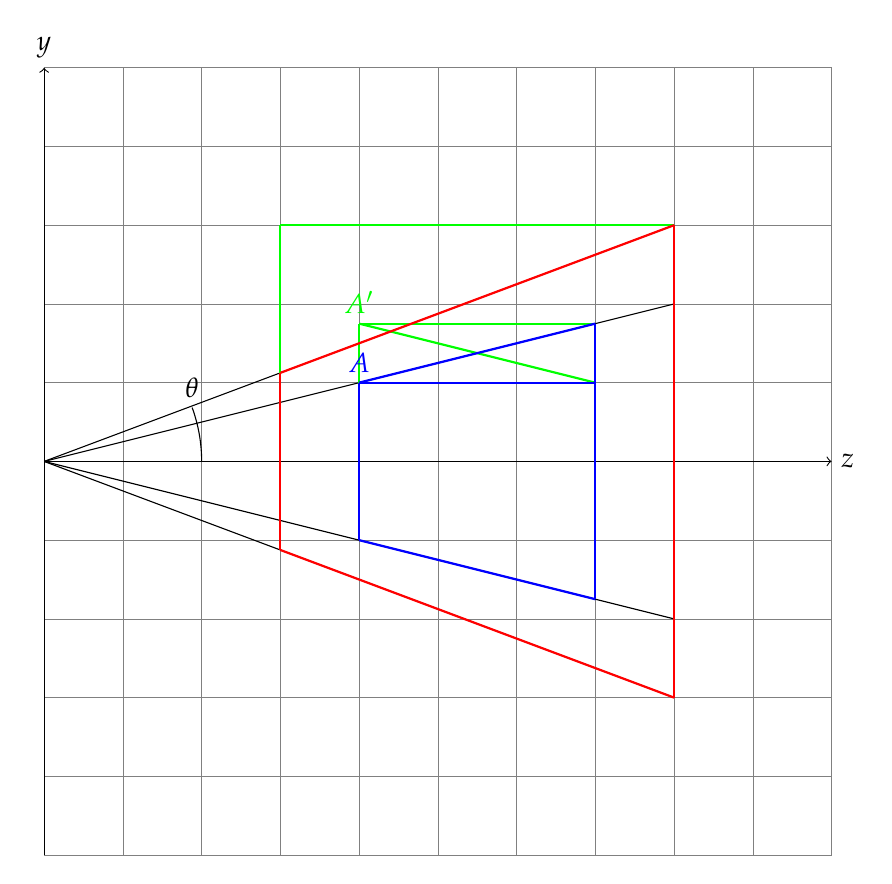
\begin{tikzpicture}[node distance=2cm]
		\draw[step=1cm,gray,very thin] (-5, -5) grid (5,5);
		\draw[->](-5,0)--(5,0) node[anchor=west] {$z$};
		\draw[->](-5,-5)--(-5,5) node[anchor=south] {$y$};
		\draw[-](-5,0)--(3,3) ;
		\draw[-](-5,0)--(3,-3) ;
		\draw[-](-5,0)--(3,-2) ;
		\draw[-](-5,0)--(3,2) ;

		\draw[-, green, thick](-2,0)--(-2,3)  ;
		\draw[-, green, thick](-1,0)--(-1,1.75) node[anchor=south] {$A'$};
		\draw[-, green, thick](-2,3)--(3,3) ;
		\draw[-, green, thick](-1,1.75)--(2,1.75);
		\draw[-, green, thick](-1,1.75)--(2,1) ;

		\draw[-, red, thick](3,-3)--(3,3) ;
		\draw[-, red, thick](-2,1.125)--(3,3) ;
		\draw[-, red, thick](-2,-1.125)--(3,-3);
		\draw[-, red, thick](-2,-1.125)--(-2,1.125);
		\draw[-, blue, thick](2,-1.75)--(2,1.75) ;
		\draw[-, blue, thick](-1,1)--(2,1.75) ;
		\draw[-, blue, thick](-1,1)--(2,1) ;
		\draw[-, blue, thick](-1,-1)--(2,-1.75) ;
		\draw[-, blue, thick](-1,-1)--(-1,1)  node[anchor=south] {$A$};
		\draw (-3,0) arc [start angle=0, end angle=20, radius=2]node[anchor=south] {$\theta$};

	\end{tikzpicture}
	\caption{$x$ 分量,与 $l,r$ 的映射关系}
	\label{Persp}
	\vspace{-2ex}
\end{figure}

在上图中,红线的是视域,蓝线是三维中的点组成的形体。现在在近平面上,我们将它缩放到和远平面一样大,此时近平面显示为绿色。类似的对于每个蓝色的点,将它所处的那个视域Z平面都缩放到和远平面一样大,显示为绿色。

可以看到处于与原点连线同一直线上的点在操作后被映射到了同一Z方向的直线上,而原本在同一Z方向的直线上的点在操作后则变为一根近大远小的绿线。可见只要对每个点做上述操作后在进行正交投影,就是我们需要的透视投影的结果。

以 $A$ 为例,在 $y$ 份量上的映射关系为:
\begin{equation*}
	\tan(\theta)=\frac{A_y}{A_z}
\end{equation*}

$A$ 所在Z平面的上端坐标 $Z_y$:
\begin{equation*}
	Z_y = A_z \tan(\theta)
\end{equation*}

远平面的上端坐标 $F_y$:
\begin{equation*}
	F_y = f \tan(\theta)
\end{equation*}

易得:
\begin{equation*}
	\frac{A'_y}{F_y}=\frac{A_y}{Z_y}
\end{equation*}

则有:
\begin{align}
	A'_y & =\frac{A_y}{Z_y}F_y                          \notag \\
	     & =\frac{A_y}{ A_z \tan(\theta)}f \tan(\theta) \notag \\
	     & =f\frac{A_y}{ A_z }\notag
\end{align}

同理有:
\begin{align}
	A'_x & =\frac{A_x}{Z_x}F_x                          \notag \\
	     & =\frac{A_x}{ A_z \tan(\beta)}f \tan(\beta) \notag   \\
	     & =f\frac{A_x}{ A_z }\notag
\end{align}

最后完整的映射为:
\begin{equation*}
	\left\{
	\begin{array}{lr}
		x' = f \frac{x}{z} \\
		y' = f \frac{y}{z} \\
		z' = f z
	\end{array}
	\right.
	\rightarrow
	\left\{
	\begin{array}{lr}
		x'z = f x \\
		y'z = f y \\
		z'=  z
	\end{array}
	\right.
\end{equation*}

尝试将上述的映射变为矩阵形式:
\begin{equation}
	\mathbf{A'} =
	\begin{bmatrix}
		f & 0 & 0 & 0 \\
		0 & f & 0 & 0 \\
		0 & 0 & 1 & 0 \\
		0 & 0 & 1 & 0 \\
	\end{bmatrix}_{\mathbf{Persp}\rightarrow\mathbf{Orth}}
	\times
	\begin{bmatrix}
		x \\
		y \\
		z \\
		1
	\end{bmatrix}
	=\begin{bmatrix}
		x'z \\
		y'z \\
		z'  \\
		z
	\end{bmatrix}
	\label{PersptoOrth}
\end{equation}

将该矩阵与正交投影矩阵相乘:
\begin{align}
	\mathbf{Perspective} & =
	\begin{bmatrix}
		\frac{2}{w} & 0           & 0             & 0              \\
		0           & \frac{2}{h} & 0             & 0              \\
		0           & 0           & \frac{1}{f-n} & -\frac{n}{f-n} \\
		0           & 0           & 0             & 1
	\end{bmatrix}
	\times
	\begin{bmatrix}
		f & 0 & 0 & 0 \\
		0 & f & 0 & 0 \\
		0 & 0 & 1 & 0 \\
		0 & 0 & 1 & 0 \\
	\end{bmatrix} \notag \\
	                     & =
	\begin{bmatrix}
		\frac{2f}{w} & 0            & 0             & 0              \\
		0            & \frac{2f}{h} & 0             & 0              \\
		0            & 0            & \frac{1}{f-n} & -\frac{n}{f-n} \\
		0            & 0            & 1             & 0
	\end{bmatrix}\notag
\end{align}

注意上述矩阵中的 $w$ 和 $h$ 是远平面的宽高。实际上 $\frac{2f}{h}$ 即为图(\ref{Persp})中的 $\cot(\theta)$ ,常用 $fov=2\theta$ ,$aspect=\frac{w}{h}$ ,则透视投影矩阵变为:
\begin{equation*}
	\mathbf{Perspective} =
	\begin{bmatrix}
		\frac{\cot(\frac{\theta}{2})}{aspect} & 0                      & 0             & 0              \\
		0                                     & \cot(\frac{\theta}{2}) & 0             & 0              \\
		0                                     & 0                      & \frac{1}{f-n} & -\frac{n}{f-n} \\
		0                                     & 0                      & 1             & 0
	\end{bmatrix}
\end{equation*}

最后,注意到公式(\ref{PersptoOrth})中的矩阵 $\mathbf{Persp}\rightarrow\mathbf{Orth}$ 的变换结果为 $x'_z, y'_z$ ,因此在计算完 $\mathbf{N}=\mathbf{Perspective}\times\mathbf{P}$ 后, $\frac{N_x}{N_w}, \frac{N_y}{N_w}$ 才是最终的结果。
\section{相机视口变换}
\subsection{世界坐标系}
在第二章中讲到的两种投影变换都是按照相机位于三维空间原点,朝向Z轴方向,Y轴向上,X轴向右的情况下得到的。但在实际的实现中,我们往往希望相机也能作为一个三维物体进行移动、旋转等变换。这就使得我们不能直接按照三维点关于原三维空间的坐标进行投影变换。
\subsection{视口坐标系}
换而言之,需要进行投影操作的点的坐标实际上是该点在以相机为原点,按相机朝向旋转后的基向量组成的坐标系,这里称为“视口坐标系”。我了能够正确的实现从相机获得的画面,我们需要对点的世界坐标进行变换。
\subsection{坐标系变换}
可知相机有旋转和平移变换,将这一变换记作 $\mathbf{C}$ ,则有视口坐标系基向量组成的矩阵 $B$:
\begin{equation*}
	\mathbf{C}\mathbf{I}=\mathbf{B}
\end{equation*}
\begin{equation*}
	\mathbf{C}=\mathbf{B}
\end{equation*}

而对于三维世界坐标系中的一点 $\mathbf{P}$ ,其视口坐标为 $\mathbf{P'}$ ,则有:
\begin{equation*}
	\mathbf{BP'}=\mathbf{P}
\end{equation*}

两边同左乘 $\mathbf{B^{-1}}$
\begin{align}
	\mathbf{B^{-1}BP'} & =\mathbf{B^{-1}P}\notag \\
	\mathbf{P'}        & =\mathbf{B^{-1}P}\notag \\
	                   & =\mathbf{C^{-1}P}
	\label{ViewMatrix}
\end{align}

其中称式(\ref{ViewMatrix})中的 $\mathbf{C^{-1}}$ 为视口变换矩阵。

综上,在将点进行投影之前,首先要计算 $\mathbf{P'}=\mathbf{C^{-1}P}$ ,后将 $\mathbf{P'}$ 作为需要变换的点即可。矩阵的逆的算法不是本次项目的重点,这里不做介绍,可见 $sunMatLib.h$ 文件。
\section{绘制/光栅化}
\subsection{三角填充}
\subsection{绘制顺序问题}
\subsection{画家算法}
\subsubsection{画家算法的问题}
\subsubsection{改进方向}
\newpage
\section{三维裁剪}
\subsection{性能问题与原因}
在上述的功能实现后,程序已经能够正确地绘制三维网格模型了,但在我们将摄像机靠近模型时,我们会发现性能的快速下降。在十分靠近模型的时候还会出现“卡死”的情况。

该问题的原因十分简单,虽然在投影一章中我们设置了远近两个平面,但在这两个平面以外的点实际上只是 $z$ 分量不在 $[0,1]$ 的区间中,他们仍会参与绘制。在正交投影中还不能看出这有什么问题,但在透视投影中,在视口坐标系Z轴正半轴区域内的点,越靠近原点,由于近大远小的原因,投影后的坐标在屏幕坐标系中将变得很大,此时三角面的光栅化将难以运行。

因此我们只希望渲染近平面以外的视域中的三角面(不考虑远平面),但在光栅化的过程中时以三角面为单位,单纯判断整个三角面是否在视域外无法解决上述的性能问题,而单纯判断三角面是否有顶点在视域外又会造成整个三角面不被渲染,从而导致模型“破损”,因此我们需要对三角面进行裁剪,对于每个面只保留在视域中的部分。
\subsection{三角面裁剪}
在三维空间中对三角面的裁剪如下图(\ref{Cut}),是一个三角面关于一张三维空间中平面的裁剪。
\begin{figure}[H]
	\centering
	\includegraphics[scale=0.4]{Picture/Annotation 2020-06-23 205119.png}
	\vspace{-2ex}
	\caption{正交投影 $vs$ 透视投影}
	\label{Cut}
\end{figure}

以平面法向的正方向表示要保留的区域,则会出现四种情况:
\begin{enumerate}
	\item 整个三角面都在保留区内
	\item 整个三角面都在保留区外
	\item 有1个顶点在保留区外,此时要保留的部分是2个三角面
	\item 有2个顶点在保留区外,此时要保留的部分是1个三角面
\end{enumerate}

首先引入“有向距离” $distance(\mathbf{P_n})$ 是空间中一点 $\mathbf{P_n}$ 到一张平面的垂直距离,在保留区内为正,否则为负。

显然, $distance<0$ 的点在保留区外。对于三角面的每个顶点 $\mathbf{P_n}$(按顺时针顺序处理),当 $distance(\mathbf{P_n}) < 0$ ,将 $\mathbf{P_n}$ 放入 $outside$ 数组,否则放入 $inside$ 数组。

当 $inside$ 数组长度为 $3$ 时对应情况1,返回原三角面。

当 $inside$ 数组长度为 $0$ 时对应情况2,返回空。

当 $inside$ 数组长度为 $1$ ,$outside$ 数组长度为 $2$ 时对应情况4,此时计算 $outside[0]$ 与 $inside[0]$ 连线与裁剪面的交点 $N_0$ ,计算 $outside[1]$ 与 $inside[0]$ 连线与裁剪面的交点 $N_1$。显然 $outside[0], outside[1], inside[0]$ 是逆时针排列的,则 $N_0, N_1, inside[0]$ 也是逆时针排列的,即裁剪后的新三角面 $TriFace(N_0, N_1, inside[0])$ 保持了原三角面的朝向。

当 $inside$ 数组长度为 $2$ ,$outside$ 数组长度为 $1$ 时对应情况3,此时计算 $outside[0]$ 与 $inside[0]$ 连线与裁剪面的交点 $N_0$ ,计算 $outside[0]$ 与 $inside[1]$ 连线与裁剪面的交点 $N_1$。显然 $inside[0], inside[1], outside[0]$ 是逆时针排列的,则 $inside[0], inside[1], N_0$ 也是逆时针排列的,即裁剪后的新三角面 $TriFace(inside[0], $
$inside[1], N_0)$ 保持了原三角面的朝向。而 $inside[1], N_0, N_1$ 也是逆时针排列的,即裁剪后的第二个三角面 $TriFace(inside[0], N_0, N_1)$ 也保持了原三角面的朝向。

$sunMatLib.h$ 中的 $Plane$ 类实现了上述裁剪算法,代码如下:
\newline
\begin{lstlisting}[language=c++]
int clip_TriFace(TriFace &in, TriFace &out1, TriFace &out2) const
{
	Vector3 *inside_point[3];
	int inside_count = 0;
	Vector3 *outside_point[3];
	int outside_count = 0;
	double d0 = distance(in.get_Point1());
	double d1 = distance(in.get_Point2());
	double d2 = distance(in.get_Point3());
	if (d0 >= 0)
	{
		inside_point[inside_count++] = &in.get_Point1();
	}
	else
	{
		outside_point[outside_count++] = &in.get_Point1();
	}
	if (d1 >= 0)
	{
		inside_point[inside_count++] = &in.get_Point2();
	}
	else
	{
		outside_point[outside_count++] = &in.get_Point2();
	}
	if (d2 >= 0)
	{
		inside_point[inside_count++] = &in.get_Point3();
	}
	else
	{
		outside_point[outside_count++] = &in.get_Point3();
	}
	if (inside_count == 0)
	{
		// No remain triface
		return 0;
	}
	if (inside_count == 3)
	{
		// origin triface
		out1 = in;
		return 1;
	}
	if (inside_count == 1 && outside_count == 2)
	{
		// one remain triface
		Vector3 p2 = intersect_Line(*inside_point[0], *outside_point[0]);
		Vector3 p3 = intersect_Line(*inside_point[0], *outside_point[1]);
		out1.set(*inside_point[0], p2, p3);
		return 1;
	}
	if (inside_count == 2 && outside_count == 1)
	{
		// two new triface
		Vector3 p12 = intersect_Line(*inside_point[0], *outside_point[0]);
		out1.set(*inside_point[0], *inside_point[1], p12);
		Vector3 p22 = intersect_Line(*inside_point[1], *outside_point[0]);
		out2.set(*inside_point[1], p12, p22);
		return 2;
	}
}
\end{lstlisting}

\subsubsection{近平面裁剪}
在有了上述的平面裁剪算法后实现近平面算法实现就很简单了。首先实例化一个 $Plane$ 类,其坐标为 $(0,0,n)$ ,法向为Z轴方向 $(0,0,1)$ 。在一个三角面执行了视口变换后,将变换后的三角面执行关于近平面的裁剪算法,将得到的结果放入投影数组即可。
\subsubsection{视口裁剪}
视口裁剪在投影前和投影后都可以实现。投影前的裁剪和近平面裁剪类似,将近平面裁剪的结果放入裁剪队列,然后对于上下左右四个视域侧面的裁剪面,进行裁剪操作,每次都将上次的裁剪结果作为带裁剪数据。从而实现视域的裁剪。这种裁剪由于视域是一个锥体,所以上下左右裁剪面的法向较难计算。

在投影后相当于在正交投影的视域内裁剪,步骤和上述裁剪一致,只是上下左右裁剪面是固定值,计算较为便利。

在我们的程序使用后者进行视口裁剪:
\newline
\begin{lstlisting}[language=c++]
TriFace clipped[2];
int new_count = 1;
std::list<TriFace> trifacelist;
trifacelist.push_back(face);
for (int p = 0; p < 4; p++)
{
	int new_tri = 0;
	while (new_count > 0)
	{
		TriFace test = trifacelist.front();
		trifacelist.pop_front();
		new_count--;
		if (p == 0) //top
		{
			const Vector3 pos(0, -1, 0);
			const Vector3 normal(0, 1, 0);
			Plane clip_plane(pos, normal);
			new_tri = clip_plane.clip_TriFace(test, clipped[0],clipped[1]);
		}
		else if (p == 1) //bottom
		{
			const Vector3 pos(0, 1, 0);
			const Vector3 normal(0, -1, 0);
			Plane clip_plane(pos, normal);
			new_tri = clip_plane.clip_TriFace(test, clipped[0],clipped[1]);
		}
		else if (p == 2) //left
		{
			const Vector3 pos(-1, 0, 0);
			const Vector3 normal(1, 0, 0);
			Plane clip_plane(pos, normal);
			new_tri = clip_plane.clip_TriFace(test, clipped[0],clipped[1]);
		}
		else if (p == 3) //right
		{
			const Vector3 pos(1, 0, 0);
			const Vector3 normal(-1, 0, 0);
			Plane clip_plane(pos, normal);
			new_tri = clip_plane.clip_TriFace(test, clipped[0],clipped[1]);
		}
		for (int i = 0; i < new_tri; i++)
		{
			trifacelist.push_back(clipped[i]);
		}
	}
	new_count = trifacelist.size();
}
\end{lstlisting}
\section{基础光照}
\subsection{全局光照}
\subsection{方向光}
\end{document}
